\documentclass[UTF8]{article} 
\usepackage[zihao=-4]{ctex}
\usepackage{graphicx}
\usepackage{amsmath, amssymb}
\usepackage{float}          
\usepackage{gbt7714} 
\usepackage{appendix}  
\usepackage{listings}     
\usepackage{hyperref}
\usepackage{CJK, CJKnumb}
\usepackage[left=30mm, right=30mm, top=35mm, bottom=35mm]{geometry} 
\usepackage{subfig}         
\usepackage{booktabs}       
\usepackage{natbib}
\setcitestyle{super,square} 

% 标题与作者信息
\title{\textbf{深度学习研究综述}} % 填写标题
\author{{U202414169 李明皓}\\
{\small 人工智能 2401 班}\\
\small 华中科技大学,人工智能与自动化学院,湖北武汉 430074}
\date{}
\begin{document}
	\maketitle
	\renewcommand{\abstractname}{}
	\begin{abstract}
		\noindent
		\textbf{摘要:}
深度学习作为一种新兴的多层神经网络训练方法,因其有效缓解了传统算法易陷入局部最优解的难题,在机器学习领域引发了广泛关注。本文首先阐述深度学习的兴起背景,深入剖析其性能优势;随后介绍当前主流的深度学习模型及其实际应用现状;最后,总结该技术领域存在的挑战与未来发展趋势。\\
		\noindent
		\textbf{关键词:} 深度学习;分布式表示;深信度网络;卷积神经网络;深凸网络 % 填写关键词
	\end{abstract}
	
	\renewcommand{\abstractname}{}
		\begin{abstract}
			\begin{center}
			\textbf{Overview of Deep Learning} \\[0.5em]
			\textbf{Li Minghao} \\[1em]
			\end{center}
		\noindent
		\textbf{Abstract:} 
	  	Deep learning is a new way of training multi-layer neural network. The optimization difficulty associated with the deep models can be alleviated, it has induced great attention of machine learning community. Firstly, this paper discussed the origin of deep learning, then analyzed virtue brought by deep learning. It introduced the main stream deep learning algorithm and their applications. Finally it concluded the problem remaining and development orientation.\\[1em]
		\noindent
		\textbf{Key words:} deep learning; distributed representation; deep belief network; convolutional neural network; deep convex network
	\end{abstract}
	\clearpage
	% 正文部分
	\section{引言}
	% 填写引言内容
	深度学习的概念源于人工神经网络的研究,含多隐层的多层感知器(MLP)就是一种深度学习结构。深度学习通过组合低层特征形成更加抽象的高层表示(属性类别或特征) ,以发现数据的分布式特征表示\cite{v1}。BP算法作为传统训练多层网络的典型算法,实际上对于仅含几层网络,该训练方法就已很不
	理想\cite{v2}。深度结构(涉及多个非线性处理单元层) 非凸目标代价函数中普遍存在的局部最小是训练困难的主要来源。
	
	Hinton\cite{v3,v4,v5}等人基于深信度网(DBN)提出非监督贪心逐层训练算法,为解决深层结构相关的优化难题带来希望,随后提出多层自动编码器深层结构。此外Lecun等人提出的卷积神经网络(CNNs)是第一个真正多层结构学习算法\cite{v6},它利用空间相对关系减少参数数目以提高BP训练性能。此外深度学习还出现许多变形结构如去噪自动编码器\cite{v7}、DCN\cite{v8}、sum-product\cite{v9}等。
	
	当前多数分类、回归等学习方法为浅层结构算法,其局限性在于有限样本和计算单元情况下对复杂函数的表示能力有限,针对复杂分类问题其泛化能力受到一定制约\cite{v2}。深度学习可通过学习一种深层非线性网络结构,实现复杂函数逼近,表征输入数据分布式表示,并展现了强大的从少数样本集中学习数据集本质特征的能力\cite{v1,v10}。本文意在向读者介绍这一刚刚兴起的深度学习新技术。
	
	% 章节示例
	\section{深度学习神经学启示及理论依据}
	\subsection{深度学习神经学启示}
	% 填写子章节内容
	尽管人类每时每刻都要面临着大量的感知数据,却总能以
	一种灵巧方式获取值得注意的重要信息。模仿人脑那样高效
	准确地表示信息一直是人工智能研究领域的核心挑战。神经
	科学研究人员利用解剖学知识发现哺乳类动物大脑表示信息
	的方式:通过感官信号从视网膜传递到前额大脑皮质再到运动
	神经的时间,推断出大脑皮质并未直接地对数据进行特征提取
	处理,而是使接收到的刺激信号通过一个复杂的层状网络模
	型,进而获取观测数据展现的规则\cite{v11,v12,v13}。也就是说,人脑并不
	是直接根据外部世界在视网膜上投影,而是根据经聚集和分解
	过程处理后的信息来识别物体。因此视皮层的功能是对感知
	信号进行特征提取和计算,而不仅仅是简单地重现视网膜的图
	像\cite{v14}。人类感知系统这种明确的层次结构极大地降低了视觉
	系统处理的数据量,并保留了物体有用的结构信息。对于要提
	取具有潜在复杂结构规则的自然图像、视频、语音和音乐等结
	构丰富数据,深度学习能够获取其本质特征。
	
	受大脑结构分层次启发,神经网络研究人员一直致力于多
	层神经网络的研究。BP 算法是经典的梯度下降并采用随机选
	定初始值的多层网络训练算法,但因输入与输出间非线性映射
	使网络误差函数或能量函数空间是一个含多个极小点的非线
	性空间,搜索方向仅是使网络误差或能量减小的方向,因而经常收敛到局部最小,并随网络层数增加情况更加严重。理论和
	实验表明 BP 算法不适于训练具有多隐层单元的深度结构\cite{v15}。
	此原因在一定程度上阻碍了深度学习的发展,并将大多数机器
	学习和信号处理研究从神经网络转移到相对较容易训练的浅
	层学习结构。
	
	传统机器学习和信号处理技术探索仅含单层非线性变换
	的浅层学习结构。浅层模型的一个共性是仅含单个将原始输
	入信号转换到特定问题空间特征的简单结构。典型的浅层学
	习结构包括传统隐马尔可夫模型(HMM) 、条件随机场
	(CRFs) 、最大熵模型(MaxEnt) 、支持向量机(SVM) 、核回归及
	仅含单隐层的多层感知器(MLP) 等。
	
	\subsection{浅层结构函数表示能力的局限性} %插入公式
	% 填写子章节内容
	早期浅层结构局限性结论是关于利用逻辑门电路实现函
	数奇偶性问题。利用一个深度为$O(\log d)$的网络用$O(d)$个
	计算节点去计算一个$d$比特和的奇偶性,而对于两层网络则需
	要指数倍数目的计算单元。随后有学者指出可以利用深度
	为$K$的多项式级的逻辑门电路实现的函数,对于$K-1$层电路
	需要指数倍的计算节点。Bengio和LeCun\cite{v10}指出深度学习结构可以很
	简洁地表示复杂函数,否则一个不合适的结构模型将需要数目
	非常大的计算单元。这里简洁包含三方面内容:a) 需要数
	据量特别是带类标记的样本;b) 需要计算单元的数目;c) 需
	要人为先验知识。例如多项式$\prod_{i=1}^n\sum_{j=1}^ma_{ij}x_j$
	可以高效地
	(相对于需训练的计算单元数目) 利用$O(mn)$运算量表示成和
	积(sum-product)结构,如果表示成积和结构,将需要$O(n^m)$计
	算量。此外Braverman\cite{v16}指出存在一大类函数不能用浅层电路表
	示。这些数学结果指出了浅层学习网络的局限性,激发了利用
	深度网络对复杂函数建模的动机。
	\clearpage
	\subsection{局部表示、分布式表示和稀疏表示}
	% 填写子章节内容
	最近许多研究者已经研究了分布式表示的一个变体,它介
	于纯粹局部表示和稠密分布式表示之间——稀疏表示。它的
	思想是尽量要求所获取表示中只有少数维是有效的,使绝大多
	数维设为0或接近于0的无效维。目的是尽量找出信号的主
	要驱动源。
	
	基于模板匹配的模型可认为含两层计算单元,第一层构建
	对输入数据进行匹配的多个模板,每一匹配单元可输出一个匹
	配度;第二层采用特定机制融合第一层的输出匹配度。典型基
	于局部匹配的例子是核方法。
	
\begin{equation}
	f(x) = b + \sum_{i} \alpha_{i} K(x, x_{i})
	\tag{1}
\end{equation}
	这里$b$和$\alpha_{i}$
	形成第二计算层。
	核函数将输入$x$匹配到训练样本$x_i$,并在全局范围求和。式(1)的结果可作为
	分类器的区分类标签,或者回归预测器的预测值。利有局部核
	函数的核方法能获取泛化性能,因其利用光滑性的先验知识,
	即目标函数可利用光滑函数逼近。在监督学习中,由训练样本
	组建预测器,当输入$x$与$x_i$靠近时,输出接近$y_i$。通常
	这是合理假设,但Bengio和LeCun\cite{v10}指出当目标函数非常复杂时,这
	样的模型泛化能力很差。其原因是利用局部估计学习算法表
	示函数时,一个局部估计子将输入空间进行切分,并需要不同
	自由度参数来描述目标函数在每一区域的形状。当函数较为
	复杂时,需要利用参数进行描述的区域数目也是巨大的。固定
	核函数的这种局限性已引起基于先验知识设计核函数的研究,
	而如果缺乏足够的先验知识是否可通过学习获取一个核函数?
	该问题同样引起大量研究。Lanckriet\cite{v17} 等人提出利用半正定规划技术学习数据的核矩阵,然后利用该核矩阵获取较好的泛
	化性能。然而当学习到的核函数相互关联时,能否获取更加简
	洁的表示?深度学习即基于这种思想并通过多次网络学习输
	入样本的分布式表示,被认为是较有前景的方法。
	
	分布式表示\cite{v18}是在机器学习和神经网络研究中可以处理
	维数灾难和局部泛化限制的一个古老的思想。如图~\ref{fig:p1}所示,分
	布式表示由一系列有可能是统计独立的显著特征组成,与局部
	泛化的方法对比,基于分布式表示的可区分模式的数目与分布
	式表示的维数(学习到的特征) 是指数倍关系的。参数数目上
	的减少对统计机器学习是非常有意义的,因为不仅可以降低运
	算量,同时仅需相对较少的样本即可避免过拟合现象的发生。
	而聚类算法和最近邻算法等局部表示算法将输入空间切分如
	图~\ref{fig:p1}左侧所示,不同局部之间是互斥的,不能形成简洁的分布
	式表示。ICA、PCA和RBM等算法用较少的特征将输入空间
	切分如图~\ref{fig:p1}右侧所示,并构建分布式表示,参数数目和需要的
	样本数要比子区域的数目少得多,这也是为什么会对未观测数
	据泛化的原因。PCA和ICA可以获取输入的主要分量信息,
	但对于输出信号数目小于输入信号数目时,不能很好地解决欠
	定问题。Kramer\cite{v19}提出了利用自联想神经网络来提取数据
	的非线性主分量的方法,该学习方法的目的是通过事物的部分
	信息或者带噪声的信息来还原事物的本来信息。自联想神经
	网络的隐层节点数目少于输入节点数目时,可认为在自联想过
	程中,这些隐层能够保留数据集中的主要信息。多层神经网络
	和Boltzmann机已被用于学习分布式表征。Salakhutdinov\cite{v20}已证明
	利用DBN学习特征空间对高斯过程回归的性能进行提高。深
	度学习算法可以看成核机器学习中一个优越的特征表示方法。Bengio\cite{v2}指出单个决策树的泛化性能随目标函数变量增加而
	降低。多个树的集成(森林)比单个树更加强大,也是因为增
	加了一个第三层,并潜在地形成分布式表示,可表达与子树数
	目指数倍个的分布。
	
	\begin{figure}[htbp]
		\centering
		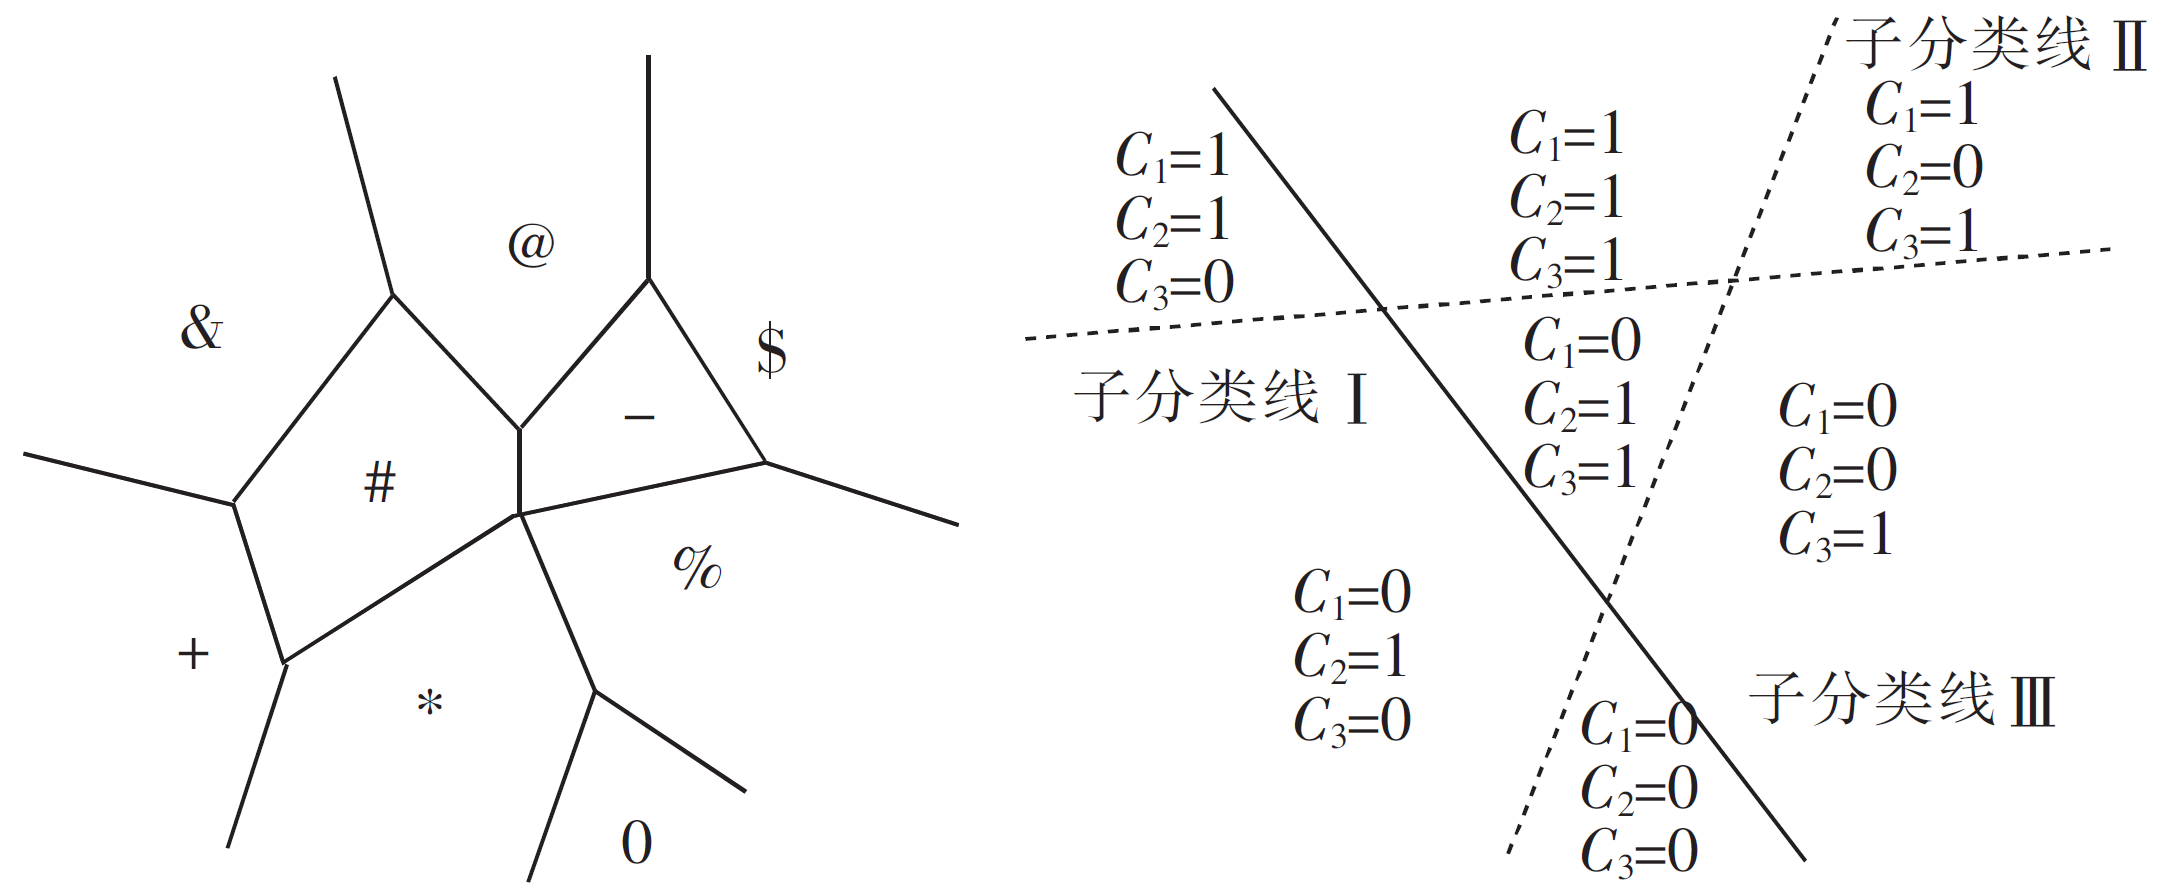
\includegraphics[scale = 0.2]{Figures/1.png} 
		\caption{数据样本的局部式表示(左)和分布式表示(右)}
		\label{fig:p1}
	\end{figure}
	
	
	\subsection{深度学习成功的关键}
	% 填写子章节内容
	深度学习具有多层非线性映射的深层结构,可以完成复杂
	的函数逼近是深度学习优势之一;此外深度学习理论上可获取
	分布式表示,即可通过逐层学习算法获取输入数据的主要驱动
	变量。该优势是通过深度学习的非监督预训练算法完成,通过
	生成性训练可避免因网络函数表达能力过强而出现过拟合情
	况。但由于单层有限的计算能力,通过多层映射单元可提取出
	主要的结构信息。Erhan等人\cite{v15}深入分析并通过实验验证了贪婪
	层次非监督深度学习方法的优势所在。
	
	\section{典型的深度学习结构}
	\subsection{生成型深度结构}
	Hinton等人\cite{v3}首次提出的DBN是目前研究和应用都比较广泛
	的深度学习结构。与传统区分型神经网络不同,可获取观测数
	据和标签的联合概率分布,这方便了先验概率和后验概率的估
	计,而区分型模型仅能对后验概率进行估计。DBN解决传统
	BP算法训练多层神经网络的难题:a) 需要大量含标签训练样本集;b)较慢的收敛速度;
c)因不合适的参数选择陷入局部
	最优。
	
	DBN由一系列受限波尔兹曼机(RBM)单元组成。RBM是一种典型神经网络,如图~\ref{fig:p2}所示。该网络可视层和隐层单元
	彼此互连(层内无连接),隐单元可获取输入可视单元的高阶
	相关性。相比传统sigmoid信度网络,RBM权值的学习相对容
	易。为了获取生成性权值,预训练采用无监督贪心逐层方式来
	实现。在训练过程中,首先将可视向量值映射给隐单元;然后
	可视单元由隐层单元重建;这些新可视单元再次映射给隐单
	元,这样就获取了新的隐单元。反复执行这种步骤叫做吉布斯
	采样。
	\begin{figure}[htbp]
	\centering
	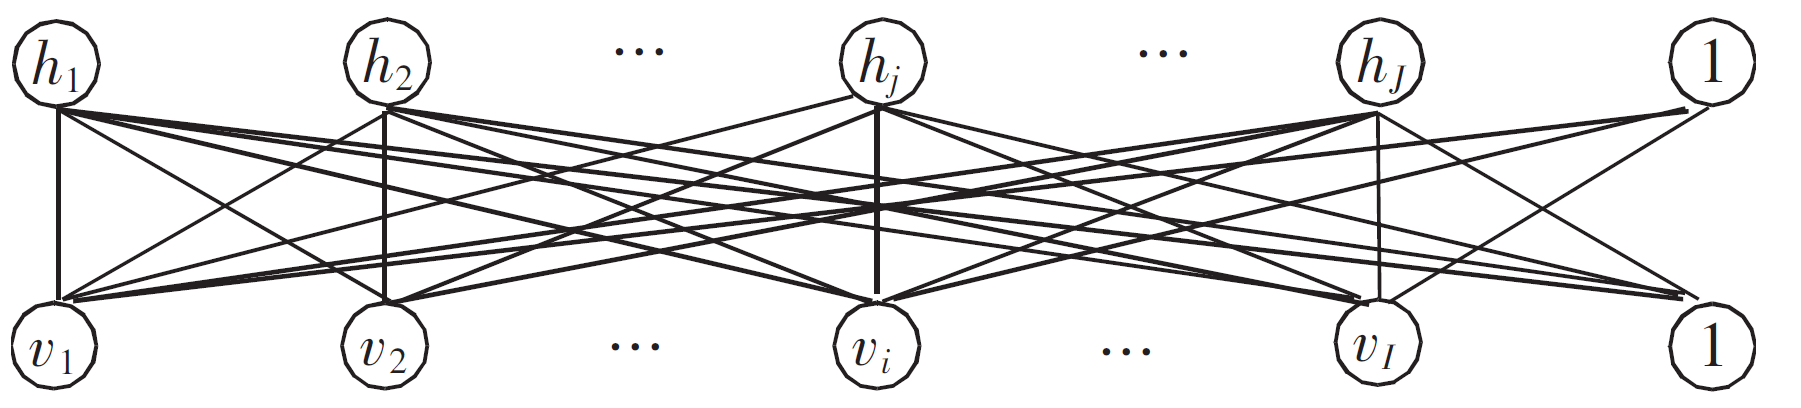
\includegraphics[scale = 0.4]{Figures/2.png} 
	\caption{RBM模块}
	\label{fig:p2}
	\end{figure}
	
RBM在给定模型参数条件下的联合分布为
\begin{equation}
	p(v,h;\theta) = \frac{\exp(-E(v,h;\theta))}{Z} 
	\tag{2}
\end{equation}
其中:\( Z = \sum_v \sum_h \exp(-E(v,h;\theta)) \)是归一化因子。
模型赋予可视向量\( v \)的边际概率为
\begin{equation}
	p(v;\theta) = \frac{\sum_h \exp(-E(v,h;\theta))}{Z}
	\tag{3}
\end{equation}
对伯努利(可视)—伯努利(隐藏)RBM能量函数定义为
\begin{equation}
	E(v,h;\theta) = -\sum_{i=1}^I \sum_{j=1}^J w_{ij}v_i h_j - \sum_{i=1}^I b_i v_i - \sum_{j=1}^J a_j h_j
	\tag{4}
\end{equation}
其中:\( w_{ij} \)为可视单元和隐单元连接权值;\( b_i \)和\( a_j \)是偏置量;\( I \)和\( J \)是可视单元和隐单元的数目。
条件概率如式(5)(6)计算:
\begin{align}
	p(h_j = 1|v;\theta) &= \delta\left( \sum_{i=1}^I w_{ij}v_i + a_j \right)
	\tag{5} \\
	p(v_i = 1|h;\theta) &= \delta\left( \sum_{j=1}^J w_{ij}h_j + b_i \right)
	\tag{6}  
\end{align}
这里\(\delta(x) = 1/(1 + \exp(x))\)。
对于高斯(可视)—伯努利(隐)RBM能量函数为
\begin{equation}
	E(v,h;\theta) = -\sum_{i=1}^I \sum_{j=1}^J w_{ij}v_i h_j + \frac{1}{2} \sum_{i=1}^I (v_i - b_i)^2 - \sum_{j=1}^J a_j h_j
	\tag{7}
\end{equation}
对应的条件概率变成:
\begin{align}
	p(h_j = 1|v;\theta) &= \delta\left( \sum_{i=1}^I w_{ij}v_i + a_j \right)
	\tag{8} \\  
	p(v_i = 1|h;\theta) &= \mathcal{N}\left( \sum_{i=1}^I w_{ij}h_j + b_i, 1 \right)
	\tag{9}  
\end{align}
	其中:\( v_i \)是满足均值为\(\sum_{j=1}^J w_{ij}h_j + b_i\),方差为1的高斯分布的实数值。高斯—伯努利RBMs可将实值随机变量转换到二进制随机变量,然后再进一步利用伯努利—伯努利RBMs处理。利用对数似然概率\(\log(p(v;\theta))\)梯度可推导出RBM的权值更新准则:
	
	\begin{equation}
		\Delta w_{ij} = E_{\text{data}}(v_i h_j) - E_{\text{model}}(v_i h_j)
		\tag{10}
	\end{equation}
	其中:\( E_{\text{data}}(v_i h_j) \)是在观测数据训练集中的期望;\( E_{\text{model}}(v_i h_j) \)是模型中定义的期望。
	
	精心训练RBM对成功应用深度学习是一个关键。Hinton\cite{v21}提供了对RBM实际训练的指导\label{sec:rbm_training}。
	通过自底向上组合多个RBM可以构建一个DBN,如图~\ref{fig:p3}
	所示。应用高斯——伯努利RBM或伯努利——伯努利RBM,可用
	隐单元的输出作为训练上层伯努利—伯努利 RBM 的输入,第
	二层伯努利和伯努利的输出作为第三层的输入等。该逐层学习策略的理论有效性已由Hinton等人(2006)\cite{v3}在《Neural Computation》中严格证明,其研究表明:这种基于伯努利RBM的逐层训练策略,能够有效提升训练数据在混合模型的似然概率的变分下界。
		
	\begin{figure}[H]
	\centering
	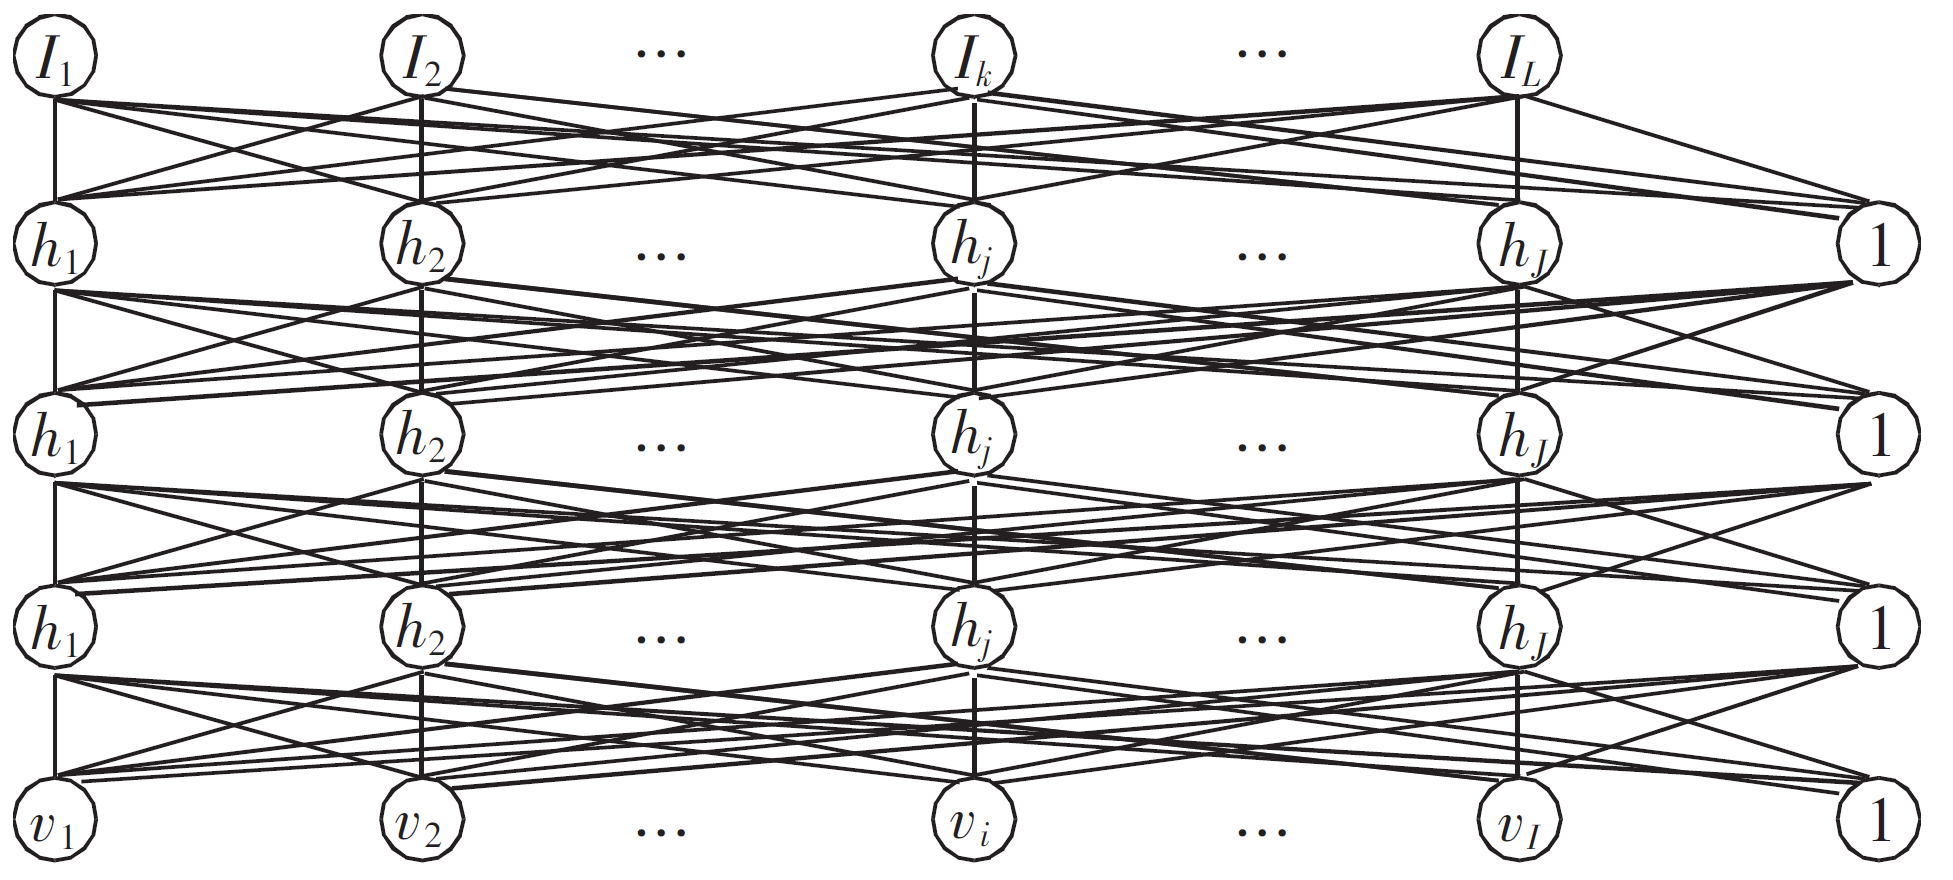
\includegraphics[scale = 0.3]{Figures/3.png} 
	\caption{DBN模型}
	\label{fig:p3}
	\end{figure}
	
	\subsection{区分性深度结构}
	卷积神经网络(CNNs)是第一个真正成功训练多层网络结
	构的学习算法,与DBNs不同,它属于区分性训练算法。受视
	觉系统结构的启示,当具有相同参数的神经元应用于前一层的
	不同位置时,一种变换不变性特征就可获取了。后来LeCun等人沿着这种思路,利用BP算法设计并训练了 CNNs。CNNs作为深度学习框架是基于最小化预处理数据要求而产生的。
	受早期的时间延迟神经网络影响,CNNs靠共享时域权值降低
	复杂度。CNNs是利用空间关系减少参数数目以提高一般前向BP训练的一种拓扑结构,并在多个实验中获取了较好性
	能\cite{v6,v22}。在CNNs中被称做局部感受区域的图像的一小部分
	作为分层结构的最底层输入。信息通过不同的网络层次进行
	传递,因此在每一层能够获取对平移、缩放和旋转不变的观测
	数据的显著特征。
	
	如Vincent等(2008)\cite{v6,v22}所述,卷积神经网络(CNNs)在MNIST手写体识别中的典型处理流程如图4所示:输入图形首先与一系列已训练的滤波器系数进行卷积操作\label{sec:cnn_conv},随后依次经过加性偏置、非线性压缩和特征归一化处理。最初阶段伴随进一步降维的下采样 $(C_{x})$ 提供对空域变化的鲁棒性;下采样特征映射经加权后的可调偏置,最终利用
	激活函数进行传递。组合多个上述映射层(图~\ref{fig:p5})可获取层间
	关系和空域信息,这样CNNs适于图像处理和理解。国内学者
	夏丁胤\cite{v23}将这种网络应用于网络图像标注中。最近CNNs已
	应用于包括人脸检测、文件分析和语音检测等不同机器学习的
	问题中。
	
	\begin{figure}[H]
	\centering
	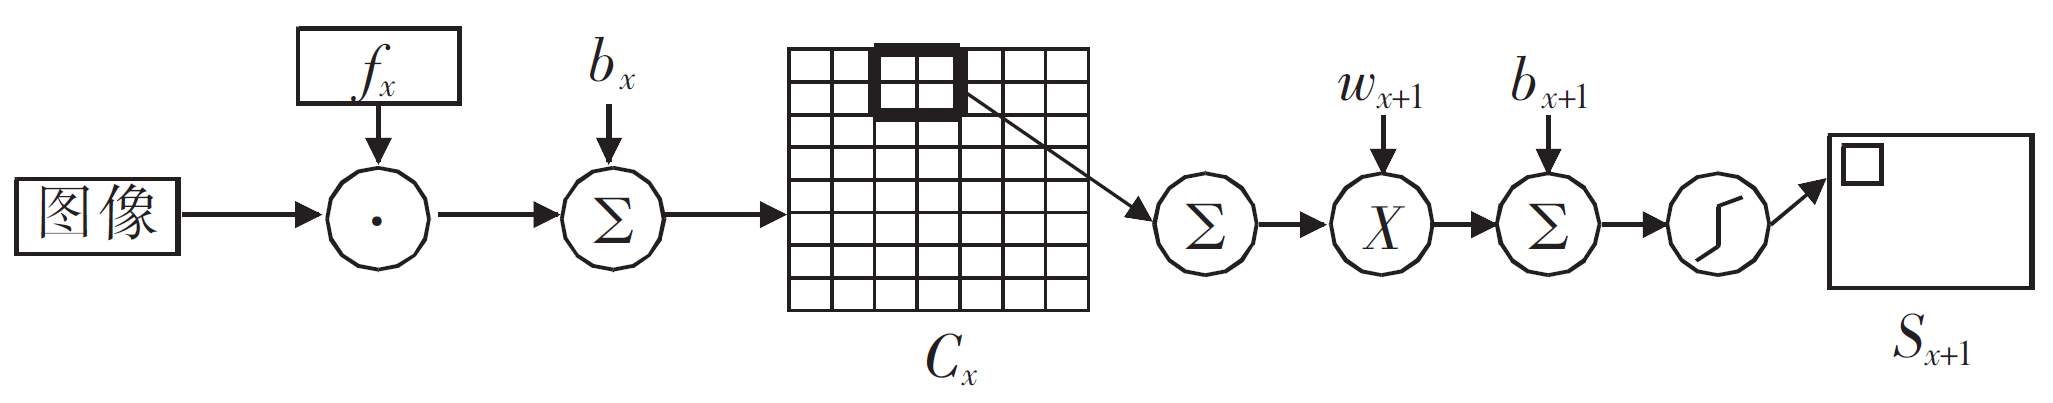
\includegraphics[scale = 0.4]{Figures/4.png} 
	\caption{CNN中卷积和采样过程}
	\label{fig:p4}
	\end{figure}
	
	\begin{figure}[H]
	\centering
	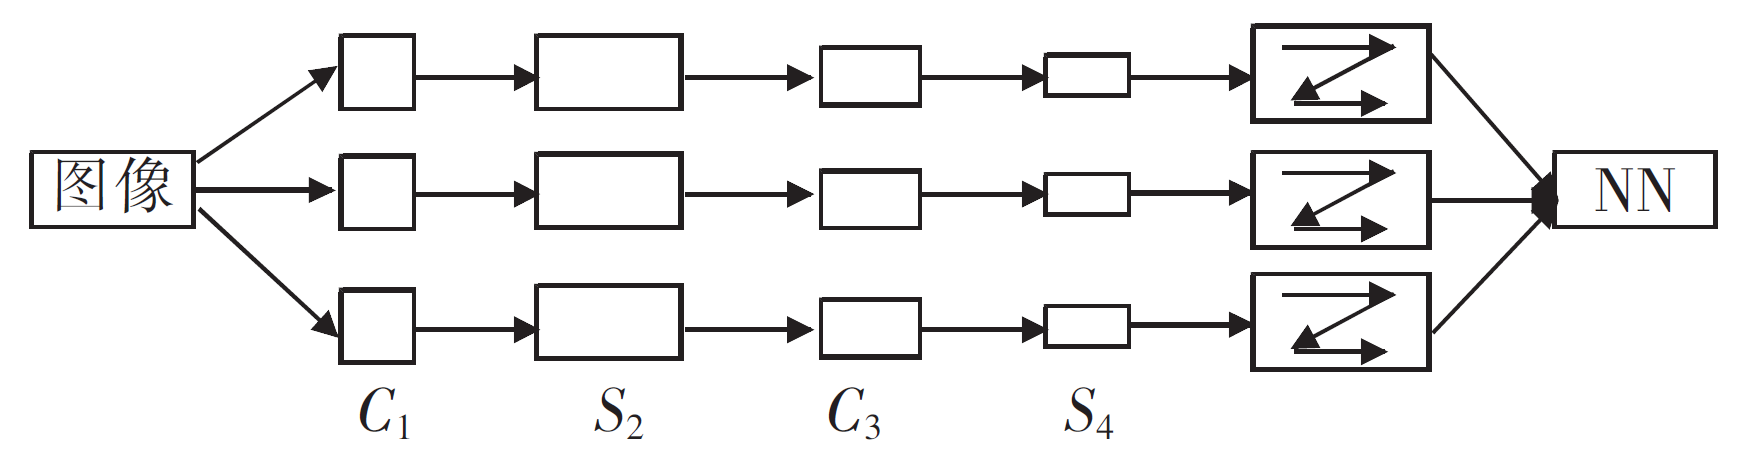
\includegraphics[scale = 0.4]{Figures/5.png} 
	\caption{卷积神经网络的原理}
	\label{fig:p5}
	\end{figure}
	
	俞栋和邓力(2011)\cite{v8}提出一新的深度学习算法。DCN如图~\ref{fig:p6}所
	示,每层子模块是含单隐层和两个可训练的加权层神经网络。
	DCN是由一系列分层子模块串联组成。模块第一个线性输入
	层对应输入特征维数,隐层是一系列非线性参数可调单元,第
	二线性输出包含线性输出单元及原始输入数据,最顶模块的输
	出代表分类目标单元。例如,如果DCN设定用于实现数字识
	别,输出可表示成1$\sim$10 的0-1编码。如用于语音识别,输入
	对应语音波形采样或波形提取特征;如功率谱或倒谱系数,输
	出单元代表不同音素。
	
	\begin{figure}[H]
	\centering
	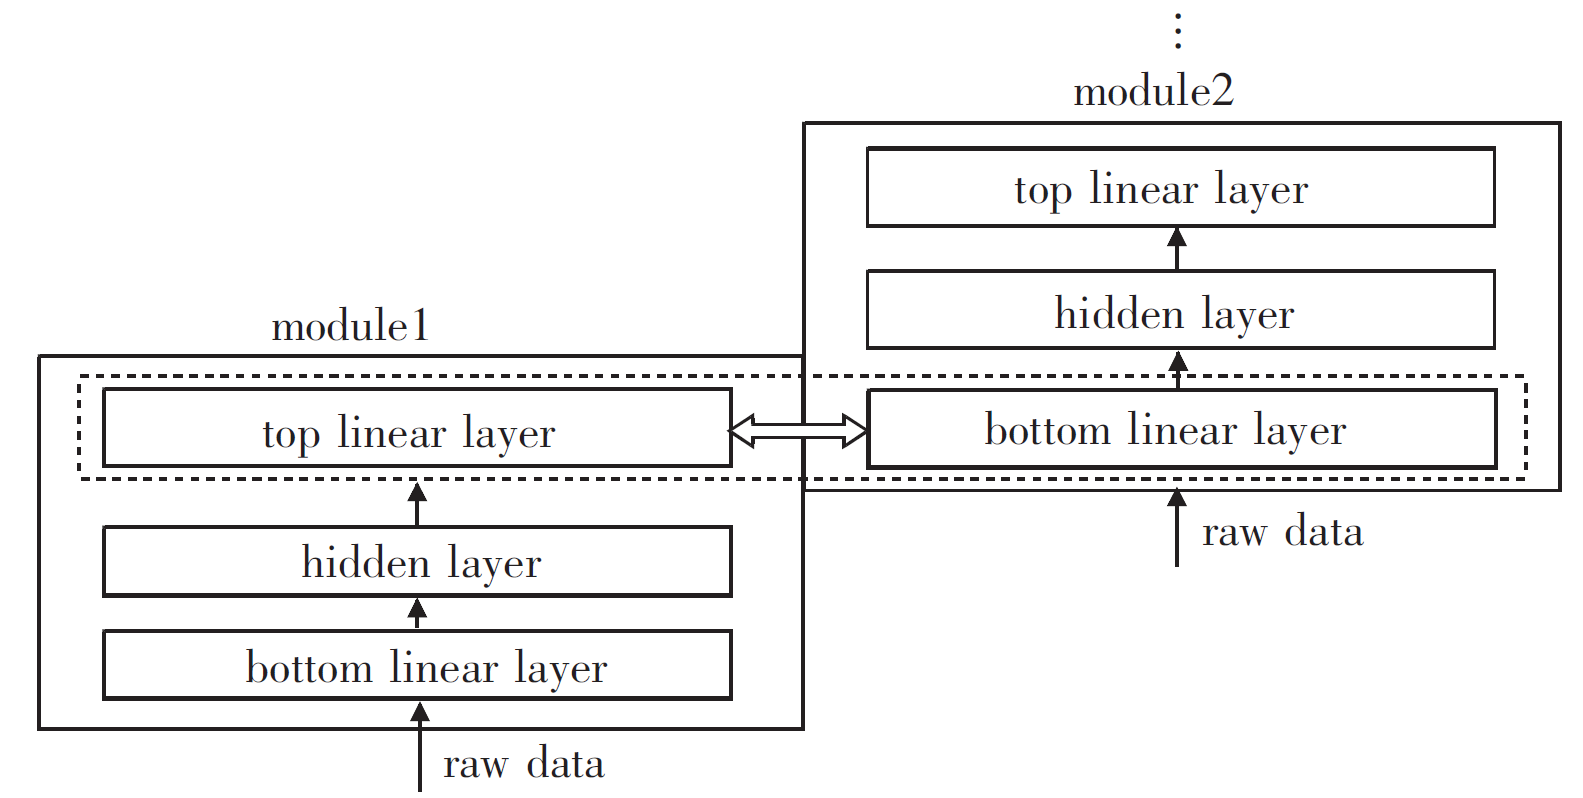
\includegraphics[scale = 0.4]{Figures/6.png} 
	\caption{DCN的结构}
	\label{fig:p6}
	\end{figure}
	
	\subsection{混合型结构}
	混合型结构的学习过程包含两个部分,即生成性部分和区
	分性部分。现有典型的生成性单元通常最终用于区分性任务,
	生成性模型应用于分类任务时,预训练可结合其他典型区分性
	学习算法对所有权值进行优化。这个区分性寻优过程通常是
	附加一个顶层变量来表示训练集提供的期望输出或标签。BP算法可用于优化DBN权值,它的初始权值通过在RBM和DBN预训练中得到而非随机产生,这样的网络通常会比仅通过BP算法单独训练的网络性能优越。可以认为BP对DBNs训练仅
	完成局部参数空间搜索,与前馈型神经网络相比加速了训练和
	收敛时间。
	
	最近,基于DBNs的研究包括应用层叠自动编码器取代传
	统DBNs中的RBMs。该方法可采用和DBNs相同的训练准
	则,不同的是自动编码器利用区分性模型。去噪自动编码器在
	训练中引入随机变化过程可以产生与传统的DBNs相比拟的
	泛化性能;对单个去噪自动编码器的训练与RBMs生成性模型
	一致。

   	\begin{table}[H]
	\centering
	\label{tab:dl_arch}
	\caption{典型深度学习结构对比}
	\begin{tabular}{p{3cm}p{3cm}p{4cm}p{3cm}}
		\toprule
		\textbf{类型}       & \textbf{核心算法}       & \textbf{特点}                          & \textbf{典型应用}         \\ 
		\midrule
		生成型(DBN)     & RBM逐层预训练         & 联合概率建模,缓解梯度消失           & 图像分类、语音识别       \\
		区分型(CNN)     & 卷积与池化操作         & 局部感受野,参数共享                 & 计算机视觉、目标检测     \\
		混合型(DBN)  & 预训练+微调            & 结合生成与区分能力,提升泛化性能     & 多模态数据融合           \\
		\bottomrule
	\end{tabular}
    \end{table}
	
	\section{深度学习应用现状}
	深度学习在信号处理中的应用对象不仅包含语音、图像和
	视频,同样也包含文本、语言和传递人类可获知的语义信息。
	传统的MLP已经在语音识别领域应用多年,在单独使用的情
	况下它们的性能远低于利用GMM-HMM的系统。
	
	最近,凭借
	具有很强区分性能力的DBNs和序列建模能力的HMMs,深度
	学习技术成功应用于语音、大词汇量连续语音识别(LVCSR)\cite{v24}
	任务。Mohamed等人(2011)\cite{v25}利用五层DBN来替换GMM-HMM中
	的高斯混合模型,并利用单音素状态作为建模单元进行语音识
	别。Nair等人(2009)\cite{v26}提出在顶层利用三阶波尔兹曼机
	的改进型DBN,并将该DBN应用于三维物体识别任务NORB数据库,给出了接近于历史最好识别误差结果,特别地,它指出DBN实质上优于SVMs等浅层模型。Fasel和Berry\cite{v27}提出了tRBM,
	并利用自动编码器对舌轮廓进行实时提取。与一般训练不同
	的是,它首先利用样本数据和人工提取的轮廓数据同时作为训练样本输入,经正常的自动编码器输出;训练完毕后,利用提出
	的tRBM对顶层进行改进,以使仅有感知图像作为输入对舌轮
	廓进行预测。
	
	此外深度学习在语言文件处理的研究日益受到
	普遍关注。利用神经网络对语言建模已有很长的历史,在语音
	识别、机器翻译、文本信息检索和自然语言处理方面具有重要
	应用。最近,深层网络已经开始吸引语言处理和信息检索方面
	的研究人员的注意。Deselaers等人(2009)\cite{v28}已利用基于DBN的多任务学习技
	术来解决机器字译问题,这可以推广到更困难的机器翻译问
	题。利用DBN和深度自动编码器对文件检索可以显示基于单
	词特征,与广泛应用的语义分析相比具有明显优势,可令文献
	检索更容易,这一思想已被初步扩展到音频文件检索和语音识
	别类问题\cite{v29}。
	
	\begin{table}[H]
		\centering
		\label{tab:dl_app}
		\caption{深度学习典型应用案例}
		\begin{tabular}{llll}
			\toprule
			\textbf{领域}       & \textbf{模型}          & \textbf{数据集}           & \textbf{性能(准确率)}  \\ 
			\midrule
			手写体识别      & LeNet-5(CNN)        & MNIST                   & 99.2\%                 \\
			语音识别        & DBN-HMM              & TIMIT                   & 83.5\%                 \\
			三维物体识别    & 改进DBN              & NORB                    & 94.8\%                 \\
			自然语言处理    & 深度自动编码器       & Penn Treebank           & 87.3\%       \\
			\bottomrule
		\end{tabular}
	\end{table}
	
	\section{结束语}
	深度学习已成功应用于多种模式分类问题。这一领域虽
	处于发展初期,但它的发展无疑会对机器学习和人工智能系统
	产生影响。同时它仍存在某些不适合处理的特定任务,譬如语
	言辨识,生成性预训练提取的特征仅能描述潜在的语音变化,
	不会包含足够的不同语言间的区分性信息;虹膜识别等每类样
	本仅含单个样本的模式分类问题也是不能很好完成的任务。
	
	深度学习目前仍有大量工作需要研究。模型方面是否有
	其他更为有效且有理论依据的深度模型学习算法,探索新的特
	征提取模型是值得深入研究的内容。此外有效的可并行训练
	算法也是值得研究的一个方向。当前基于最小批处理的随机
	梯度优化算法很难在多计算机中进行并行训练。通常办法是
	利用图形处理单元加速学习过程,然而单个机器GPU对大规
	模数据识别或相似任务数据集并不适用。在深度学习应用拓
	展方面,如何充分合理地利用深度学习在增强传统学习算法的
	性能仍是目前各领域的研究重点。
    
    
    % 参考文献
    \bibliographystyle{gbt7714-numerical}
    \bibliography{references} 
    \clearpage
    
	 % 附录
	\appendix
	\section*{附录A\ RBM的对比散度算法训练步骤}
	\label{app:cd}
	(详见正文第\ref{sec:rbm_training}节)受限玻尔兹曼机(RBM)的训练通常采用对比散度(Contrastive Divergence, CD)算法,具体步骤如下:
	\begin{enumerate}
		\item 初始化可见层状态$v^{(0)}$为训练样本。
		\item 对于$k$次吉布斯采样:
		\begin{itemize}
			\item 根据$p(h^{(t)}|v^{(t)})$采样隐层状态$h^{(t)}$。
			\item 根据$p(v^{(t+1)}|h^{(t)})$采样可见层状态$v^{(t+1)}$。
		\end{itemize}
		\item 计算参数的梯度更新:
		\[
		\Delta w_{ij} = \eta \left( \langle v_i h_j \rangle_{\text{data}} - \langle v_i h_j \rangle_{\text{recon}} \right)
		\]
其中,$\eta$为学习率。
	\end{enumerate}
	
	\section*{附录B\ 卷积神经网络中的卷积计算示例}
	\label{app:conv}
	(详见正文第\ref{sec:cnn_conv}节)考虑输入矩阵 $\mathbf{I}$ 和卷积核 $\mathbf{K}$,其卷积操作计算如下:
    \[
    (\mathbf{I} * \mathbf{K})_{i,j} = \sum_{m=0}^{M-1} \sum_{n=0}^{N-1} \mathbf{I}_{i+m, j+n} \cdot \mathbf{K}_{m,n}
    \]
    其中,$M$和$N$分别为卷积核的高度和宽度。
	
	% 致谢
	\section*{致谢}
	
衷心感谢人工智能与自动化学院开设的《文献检索与科技论文写作》课程,以及谭山老师的悉心指导与启发。通过系统的理论学习和实践训练,我掌握了科技论文撰写的核心方法与LaTeX、EndNote等专业工具的使用技巧。特别感谢学长学姐在论文写作过程中给予的宝贵经验分享,使我少走许多弯路。文中若存在疏漏或不足之处,恳请老师批评指正。
	
\end{document}
